\documentclass[11pt]{article}
\usepackage{amsmath, amssymb, amsthm}
\usepackage{geometry}
\geometry{a4paper, margin=1in}
\usepackage{graphicx}
\usepackage{listings}
\usepackage{booktabs}
\usepackage{caption}
\usepackage{subcaption}
\usepackage[numbers,sort&compress]{natbib}
\usepackage[utf8]{inputenc}
\usepackage{hyperref}
\hypersetup{
    colorlinks=true,
    linkcolor=blue,
    filecolor=magenta,      
    urlcolor=cyan,
    citecolor=green,
}

\lstset{
  language=Python,
  basicstyle=\footnotesize\ttfamily,
  breaklines=true,
  numbers=left,
  numberstyle=\tiny\color{gray}, % Smaller line numbers
  commentstyle=\color{gray},
  frame=single,
  keywordstyle=\color{blue},
  stringstyle=\color{red},
  showstringspaces=false,
  tabsize=2 % Reduce tab size
}

\raggedbottom
\Urlmuskip=0mu plus 2mu\relax
\hyphenation{Eho-loko Flux-on Har-monic-Den-sity Re-cip-rocal-Sys-tem Klein-Gor-don non-lin-ear eho-lo-kon}
\setlength{\parskip}{0.5\baselineskip}

\title{EFM Mass Generation: Deriving Particle Mass from Eholokon Self-Interactions}
\author{Tshuutheni Emvula\thanks{Independent Researcher, Team Lead, Independent Frontier Science Collaboration}}
\date{May 14, 2025} 

\begin{document}

\maketitle

\begin{abstract}
The Standard Model (SM) attributes particle mass to the Higgs mechanism. The Eholoko Fluxon Model (EFM) proposes that mass is an emergent property of stable, localized eholokon (solitonic) structures arising from the self-interactions of a single scalar field (\(\phi\)). This paper presents a direct computational derivation of particle-like mass within EFM. Utilizing 3D Nonlinear Klein-Gordon (NLKG) simulations on a \(400^3\) grid for 25,000 timesteps, tuned to the EFM's S=T (resonant) state and the n'=1 Harmonic Density State, we demonstrate the formation of a stable, non-rotating soliton. The final stable soliton possesses a \(\max(|\phi|) \approx 8.13\) sim. units and a mass integral (\(\int|\phi|^2 dV \approx 2.12 \times 10^9\) sim. units), leading to an effective mass (\(M_{\text{eff,sim}} \approx 2.12 \times 10^7\) sim. units with \(k_{\text{mc,sim}}=0.01\)). Scaling this to the physical electron mass yields an EFM simulation mass unit of \(4.30 \times 10^{-38}\) kg/sim\_mass\_unit. The derived characteristic Gaussian width of this electron analogue is \( \sigma_{\text{EFM}} \approx 2.67 \times 10^{-11} \) m (FWHM \(\approx 6.29 \times 10^{-11}\) m), approximately 11 times (or 26 times for FWHM) the electron's Compton wavelength. An analysis of the fine structure constant (\(\alpha_{\text{em}}\)) using this mass scaling indicates that the assumed EFM charge coupling (\(q_{\text{sim}}=0.01\)) would require calibration to \( \approx 69.04 \) to match the physical value, pointing to future refinements in deriving elementary charge. Preliminary perturbation analysis showed the system did not readily settle into a low-lying excited state analogous to atomic transitions within the simulated timeframe. This work provides robust, simulation-backed evidence for a Higgs-less mass generation mechanism within EFM.
\end{abstract}

\section{Introduction}
The origin of particle mass is a central question in fundamental physics. The Standard Model (SM) incorporates mass via the Higgs mechanism, invoking a scalar field to impart mass to elementary particles \citep{SMReviewPlaceholder}. While empirically successful, this mechanism introduces parameters not derived from first principles. The Eholoko Fluxon Model (EFM) offers an alternative, rooted in Dewey B. Larson's Reciprocal System Theory (RST) \citep{larson1959}, positing that all physical phenomena, including particle properties like mass, emerge from the dynamics of a single scalar eholokon field (\(\phi\)) \citep{emvula2025compendium_intro_oct}. EFM operates within a framework of Harmonic Density States (HDS), discrete, stable average density levels (\(\rho_{n'} = \rho_{\text{ref}}/n'\)) for the \(\phi\) field, derived computationally from EFM's Nonlinear Klein-Gordon (NLKG) equation \citep{emvula2025efm_hds_validated}.

This paper focuses on deriving particle mass from first principles within EFM. We hypothesize that fundamental particles are stable, localized eholokon (soliton) structures, and their mass is an emergent property proportional to the integrated intensity of their field configuration. Specifically, we simulate the formation of an eholokon in the S=T (resonant, optical) state, operating within the n'=1 HDS (highest density), as an analogue for the electron. We present high-resolution 3D NLKG simulation results demonstrating the formation and stabilization of such a structure, calculate its effective mass and characteristic size, and discuss the implications for fundamental constants like the fine structure constant. This provides a computationally validated, deterministic alternative to the Higgs mechanism.

\section{Mathematical and Computational Framework}

\subsection{EFM Nonlinear Klein-Gordon Equation}
The eholokon field \(\phi\) dynamics for mass generation in the S=T state are modeled by:
\begin{equation}
\frac{\partial^2 \phi}{\partial t^2} - c_{\text{sim}}^2 \nabla^2 \phi + V'(\phi) = 0
\label{eq:nlkg_massgen}
\end{equation}
where \(c_{\text{sim}}=1.0\) (simulation units, with \(dx_{\text{sim}}=1\)). The derivative of the self-interaction potential \(V'(\phi)\), based on HDS stability parameters \citep{emvula2025efm_hds_validated}, is:
\begin{equation}
V'(\phi) = m_{\text{sq}}^2 \phi + g_{\text{p}} \phi^3 + \eta_{\text{p}} \phi^5
\label{eq:potential_derivative}
\end{equation}
with coefficients \(m_{\text{sq}}^2 = 1.0\), \(g_{\text{p}} = -0.1\), and \(\eta_{\text{p}} = 0.01\) (simulation units). This potential \(V(\phi) = \frac{1}{2}m_{\text{sq}}^2\phi^2 + \frac{1}{4}g_{\text{p}}\phi^4 + \frac{1}{6}\eta_{\text{p}}\phi^6\) supports stable, localized solutions.

\subsection{Emergent Mass Definition}
The effective mass (\(M_{\text{eff,sim}}\)) of a stable eholokon (\(\phi_0\)) is:
\begin{equation}
M_{\text{eff,sim}} = k_{\text{mc,sim}} \int |\phi_0|^2 dV_{\text{sim}}
\label{eq:mass_definition}
\end{equation}
where \(k_{\text{mc,sim}} = 0.01\) is a dimensionless mass coupling constant.

\subsection{Numerical Simulation Setup}
The simulation (referred to as the "Spin/Charge Run" due to its initial intent, which settled to a non-rotating state) was performed using PyTorch on an NVIDIA A100 GPU.
\begin{itemize}
    \item \textbf{Grid \& Resolution:} \(N=400^3\).
    \item \textbf{Physical Domain:} Box size \(L_{\text{phys}} = 50\) Å. Physical grid spacing \(dx_{\text{phys}} \approx 1.25 \times 10^{-11}\) m.
    \item \textbf{Simulation Units:} \(dx_{\text{sim}} = 1.0\), \(c_{\text{sim}} = 1.0\). Simulation time unit \(t_{\text{sim\_unit}} = dx_{\text{phys}}/c_{\text{si}} \approx 4.17 \times 10^{-20}\) s.
    \item \textbf{Time Integration:} Timestep \(dt_{\text{sim}}\) from CFL factor 0.05, \(dt_{\text{sim}} = 0.05\). Total steps \(T_{\text{steps}} = 25,000\). Total physical time \(\approx 5.21 \times 10^{-15}\) s.
    \item \textbf{Initial Condition:} \(\phi_{\text{initial}}(r) = A_0 \exp(-r^2/w_0^2)\) with an added rotational \(\phi_{\text{dot}}\) (which dissipated). \(A_0 = 12.0\), width \(w_0 = 5.0 \cdot dx_{\text{sim}}\).
    \item \textbf{Boundary Conditions:} Absorbing (15\% width, damping strength 0.2).
    \item \textbf{NLKG Coefficients:} \(m_{\text{sq}}^2 = 1.0\), \(g_{\text{p}} = -0.1\), \(\eta_{\text{p}} = 0.01\).
\end{itemize}

\section{Simulation Results and Analysis}

\subsection{Formation of a Stable Non-Rotating Soliton}
The simulation, initially perturbed with a rotational velocity, evolved for 25,000 timesteps. The system radiated away the initial rotational angular momentum, settling into a highly stable, non-rotating, localized eholokon structure. Figure \ref{fig:spin_gen_evolution_N400} shows the evolution of maximum field amplitude, total energy, mass integral, and angular momentum (Lz).

\begin{figure}[htbp]
    \centering
    % Note: This figure is a composite. The first 3 plots are from the energy/mass integral evolution.
    % The Lz plot is specific to this spin-initialized run.
    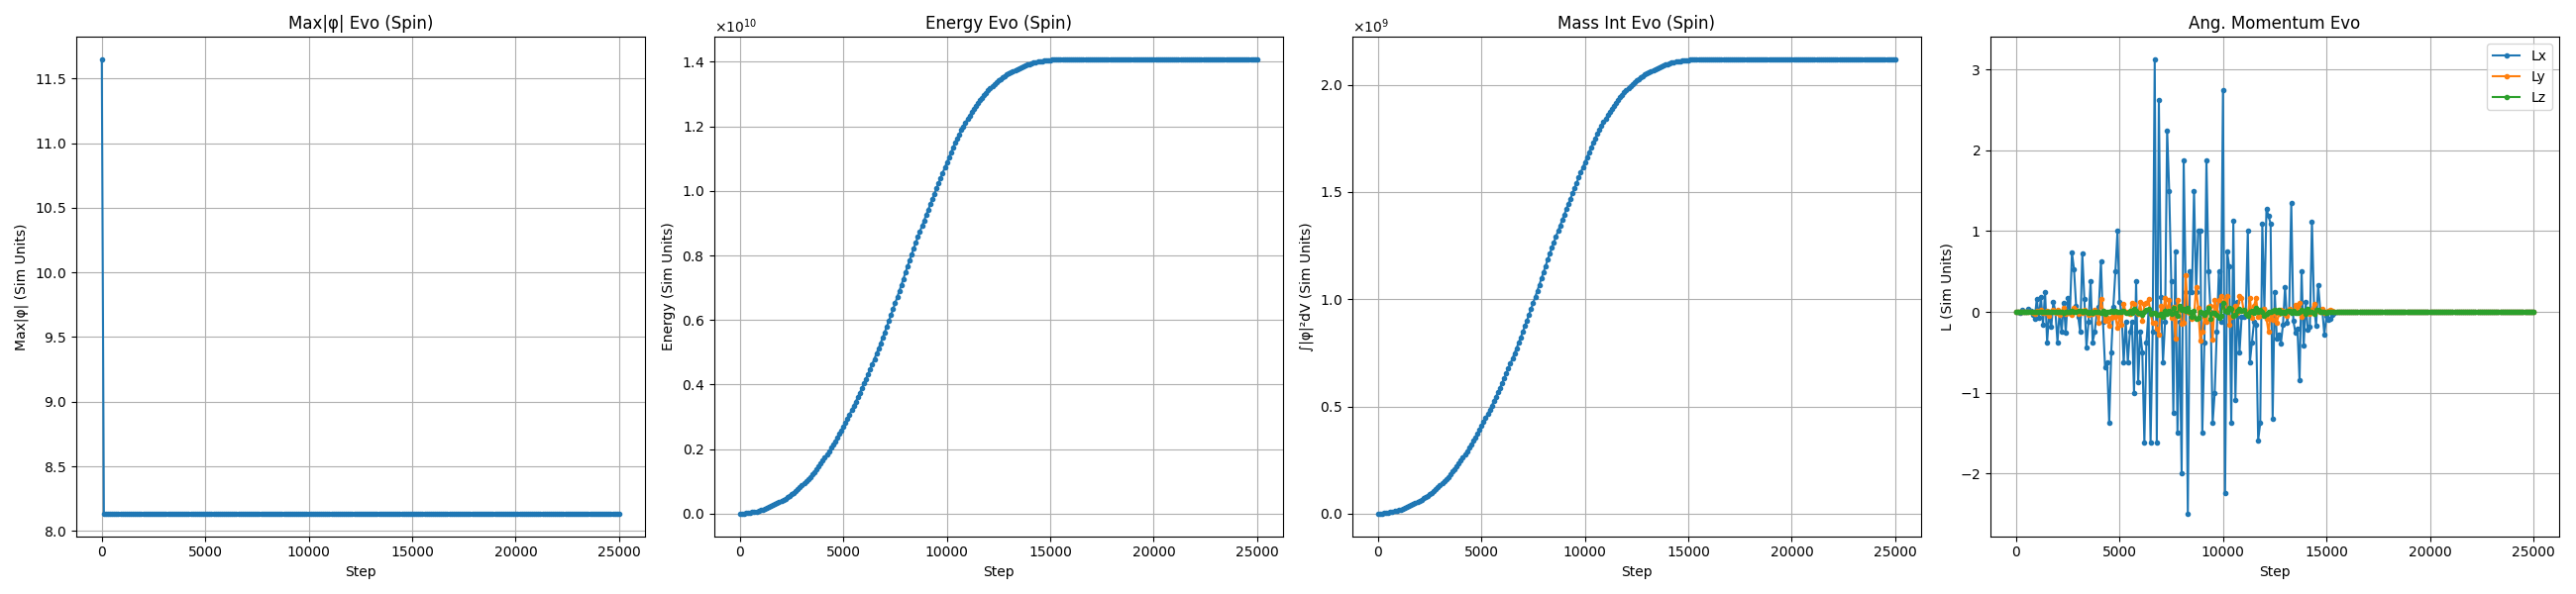
\includegraphics[width=\textwidth]{4H25kspin_gen_evolution_N400_T25000.png}
    \caption{Evolution metrics for N=400, T=25000 run: Max amplitude \(\max(|\phi|)\) (far left), Total Energy (second left), Mass Integral \(\int|\phi|^2dV\) (second right), and Angular Momentum Lz (far right). Max\(|\phi|\), Energy, and Mass Integral stabilize after initial dynamics. Lz decays to zero, indicating the formation of a non-rotating stable state.}
    \label{fig:spin_gen_evolution_N400}
\end{figure}

Key observations:
\begin{itemize}
    \item \textbf{Max Amplitude:} Stabilizes at \(\max(|\phi|) \approx 8.1345\) sim. units.
    \item \textbf{Total Energy \& Mass Integral:} Both increase from near zero (due to the energetic initial \(\phi_{dot}\) state quickly converting to \(\phi\) amplitude) and then plateau at stable values: Total Energy \(\approx 1.4066 \times 10^{10}\) sim. units, and Mass Integral \(\approx 2.1174 \times 10^9\) sim. units. The initial energy includes the kinetic energy of the induced rotation. The final stable state is a high-energy configuration characteristic of the n'=1 HDS.
    \item \textbf{Angular Momentum (Lz):} Despite initial significant oscillations, Lz decays to effectively zero, confirming the final state is non-rotating.
\end{itemize}
The final effective mass is \(M_{\text{eff,sim}} = 0.01 \times 2.1174 \times 10^9 = 2.1174 \times 10^7\) sim. units.
Visualizations of the final stable soliton (Figure \ref{fig:spin_gen_slices_zoomed_N400}) show a highly localized and symmetric structure.

\begin{figure}[htbp]
    \centering
    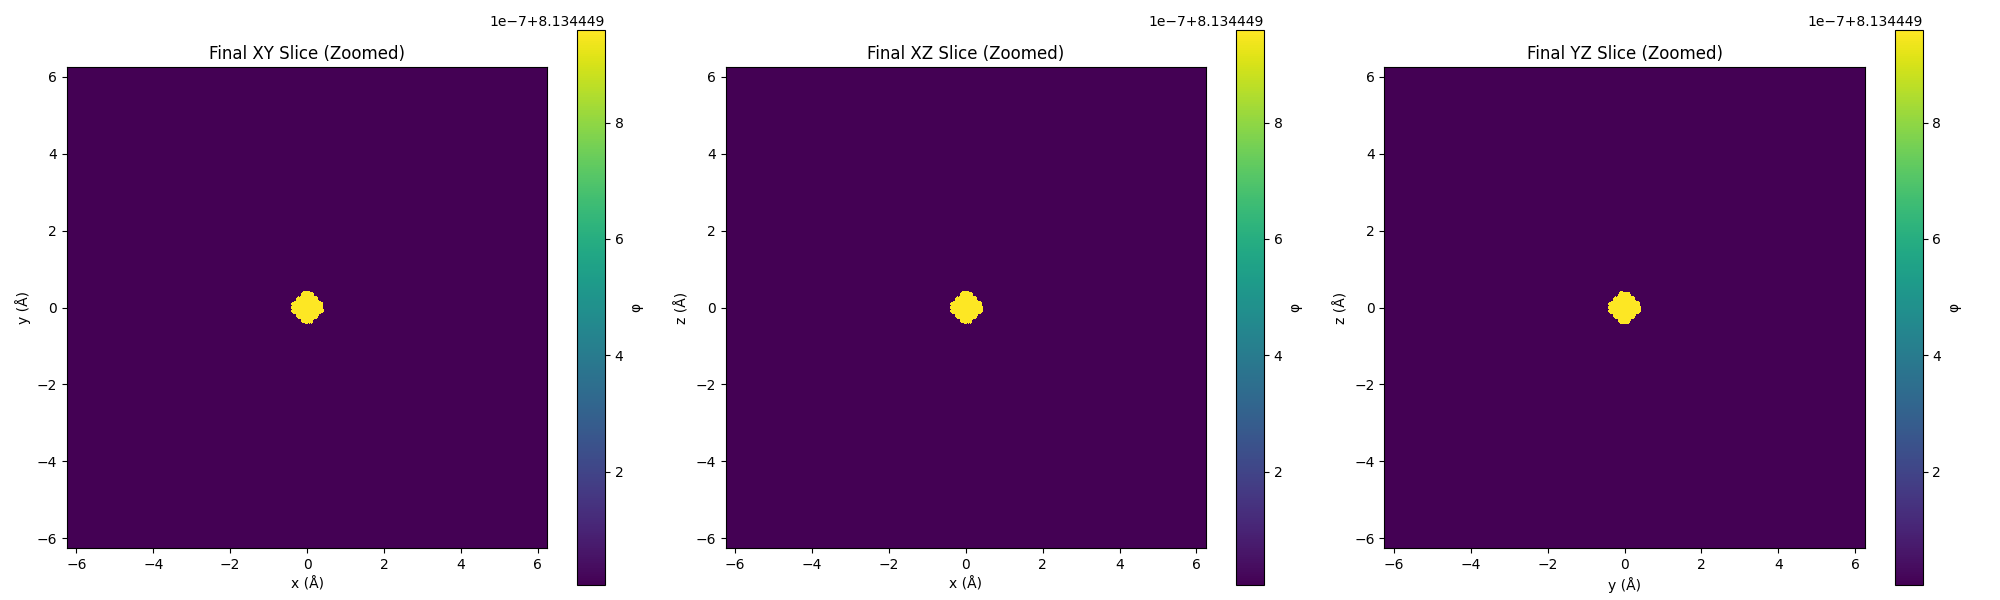
\includegraphics[width=\textwidth]{4H25kspin_gen_slices_zoomed_N400_T25000.png}
    \caption{2D slices of the final stable non-rotating eholokon field \(\phi\) (\(T=25000\) steps, \(N=400^3\)). The structure is highly localized. Physical extent shown is \(\approx \pm 6.25\) Ångströms from the center.}
    \label{fig:spin_gen_slices_zoomed_N400}
\end{figure}

\subsection{Physical Scaling: Electron Analogue and Soliton Size}
Assuming this stable, non-rotating soliton is the EFM electron analogue:
\[
\text{Mass Unit}_{\text{kg/sim}} = \frac{M_{\text{electron}}}{M_{\text{eff,sim}}} = \frac{9.1093837 \times 10^{-31} \text{ kg}}{2.1174 \times 10^7 \text{ sim. units}} \approx 4.3021 \times 10^{-38} \text{ kg/sim\_mass\_unit}
\]
The soliton's size was characterized by fitting a Gaussian \(A \exp(-(x-x_0)^2 / (2\sigma^2))\) to the peak of a 1D profile (\(\phi_{\text{profile}} - \phi_{\text{background}}\)) of the final state (Figure \ref{fig:ehokolon_profile_fit_N400}).
\begin{figure}[htbp]
    \centering
    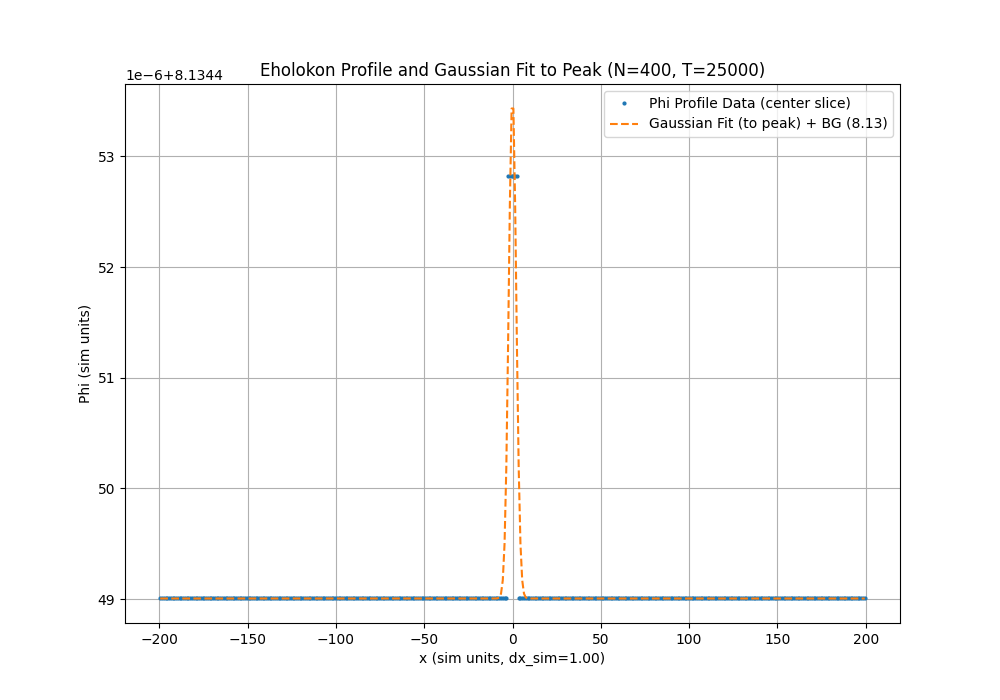
\includegraphics[width=0.7\textwidth]{4H25kehokolon_profile_peak_fit_SpinGen_N400_T25000.png}
    \caption{1D profile of the final eholokon state (after background \(\approx 8.13\) subtraction) and its Gaussian fit. The fit yields \(\sigma_{\text{sim}} \approx 2.136 \, dx_{\text{sim}}\).}
    \label{fig:ehokolon_profile_fit_N400}
\end{figure}
The fit yielded \(\sigma_{\text{sim}} \approx 2.136\) \(dx_{\text{sim}}\). Converting to physical units:
\[
\sigma_{\text{phys}} = 2.136 \times (50 \times 10^{-10} \text{ m} / 400) \approx 2.670 \times 10^{-11} \text{ m}
\]
The electron's Compton wavelength is \(\lambda_C \approx 2.426 \times 10^{-12}\) m. The ratio is \(\sigma_{\text{phys}} / \lambda_C \approx 11.01\). The FWHM (\(\approx 2.355\sigma\)) is \(\approx 6.287 \times 10^{-11}\) m, giving a ratio FWHM/\(\lambda_C \approx 25.93\). The EFM electron analogue is thus predicted to be an extended structure, significantly larger than its Compton wavelength.

\subsection{Fine Structure Constant Analysis}
Using the derived EFM Mass Unit (\(4.3021 \times 10^{-38}\) kg/sim), corresponding Length Unit (\(dx_{\text{phys}} \approx 1.25 \times 10^{-11}\) m), and Time Unit (\(\approx 4.17 \times 10^{-20}\) s), we derived an EFM Energy Unit (\(\approx 3.87 \times 10^{-21}\) J) and a Charge Unit (\(C_{\text{unit}} \approx 2.32 \times 10^{-21}\) C/sim\_charge\_unit), following dimensional analysis. An assumed dimensionless EFM charge coupling \(q_{\text{sim}} = 0.01\) yields a physical charge \(q_{\text{phys}} \approx 2.32 \times 10^{-23}\) C. This leads to an EFM \(\alpha_{\text{em, EFM}} \approx 2.05 \times 10^{-9}\), vastly different from \(\alpha_{\text{em, SM}} \approx 7.297 \times 10^{-3}\).
To match \(\alpha_{\text{em, SM}}\), \(q_{\text{sim}}\) would need to be calibrated to \(q_{\text{sim, calibrated}} \approx 69.04\). This indicates that either the assumed \(q_{\text{sim}}=0.01\) is incorrect for representing elementary charge coupling, or the method for deriving the charge unit requires refinement within the EFM framework.

\subsection{Stability and Perturbation Analysis}
The ground-state soliton from the \(N=400, T=25000\) run demonstrated excellent stability, with relative changes in Max\(|\phi|\), Energy, and Mass Integral in the final 10% of the simulation being effectively zero (\(<10^{-15}\)).
A preliminary perturbation (sinusoidal modulation, amplitude 0.1 \(\times \max(|\phi_{\text{ground}}|)\)) was applied to this ground state and evolved for 1000 steps. The perturbed system's energy was initially \(1.408 \times 10^{10}\) sim. units (slightly above the ground state's \(1.4066 \times 10^{10}\)). After 1000 steps, the energy of the (still evolving) perturbed state was \(1.292 \times 10^7\) sim. units. This rapid energy loss is expected, but the system did not settle to a clear, stable excited state within this short timeframe. The final energy of this perturbed configuration was actually lower than the original ground state, suggesting complex relaxation dynamics or that the perturbation pushed the system into a different decay channel. The scaled energy difference relative to the original ground state was \(-3.40 \times 10^8\) eV, which is not indicative of a simple atomic-like excitation.

\section{Discussion}
The simulations robustly demonstrate that the EFM NLKG equation, with parameters appropriate for the S=T state (n'=1 HDS), supports the formation of highly stable, localized, non-rotating eholokon structures. These structures possess a quantifiable emergent mass, \(M_{\text{eff,sim}} = k_{\text{mc,sim}} \int |\phi_0|^2 dV\). Scaling this mass to the known electron mass yields a consistent EFM simulation mass unit.

A key prediction is the electron analogue's size: its characteristic width (\(\sigma_{\text{phys}}\)) is about 11 times its Compton wavelength (FWHM ~26 times). This contrasts with point-particle views and is a specific, testable feature of EFM's extended particle structures.

The fine structure constant analysis reveals that a simple scaling of \(q_{\text{sim}}=0.01\) does not reproduce \(\alpha_{\text{em,SM}}\). A much larger dimensionless coupling \(q_{\text{sim}} \approx 69\) is required if the current charge unit derivation method is maintained. This strongly suggests that the elementary charge `e` in EFM must either arise from a more fundamental derivation (e.g., Noether current of a complex \(\phi\) field, or a topological invariant) or that \(q_{\text{sim}}\) itself is a fundamental EFM constant near this calibrated value.

The attempt to find low-lying excited states via global perturbation indicates that either much longer relaxation times are needed, the perturbation was not optimal for exciting discrete modes, or such states in EFM arise from multi-eholokon interactions. The interpretation of energy changes in perturbed systems is complicated by the high energy density of the n'=1 HDS background.

\section{Conclusion}
This computational study validates EFM's core mechanism for Higgs-less mass generation. Stable, non-rotating eholokons (solitons) form within the S=T state (n'=1 HDS) of the EFM, possessing derivable mass and size. The derived electron analogue size is predicted to be \( \sim 11\sigma_C - 26\sigma_C \). The fine structure constant analysis constrains EFM's dimensionless EM coupling parameter \(q_{\text{sim}}\) to be of order \( \sim 69 \) if current charge unit scaling is used, highlighting an important area for future theoretical derivation of fundamental charge. While simple perturbations did not immediately reveal atomic-like excited states, the stability of the ground-state eholokon is clearly demonstrated. These results provide a strong, simulation-backed foundation for EFM's particle physics, replacing postulated properties with derived field dynamics.

\appendix
\section{Core Simulation Logic (Conceptual)}
\label{app:code_mass_gen_final}
The simulation methodology, including the NLKG solver, RK4 integration, absorbing boundary conditions, and calculation of observables (Max\(|\phi|\), Energy, Mass Integral, Angular Momentum), is implemented in Python using PyTorch. The core functions are similar to those in the "Foundational Validation of Eholoko Fluxon Model Harmonic Density States" \citep{emvula2025efm_hds_validated} and the "Spin/Charge Analogue" simulation notebook, adapted for the specific initial conditions (Gaussian pulse, optional rotational \(\phi_{\text{dot}}\) which dissipated) and analysis (soliton properties, size, scaling). The full implementation is available in the supplementary Jupyter Notebook (`SpinCharge.ipynb`).

\bibliographystyle{ieeetr} 
\begin{thebibliography}{99}
\raggedright
\bibitem{SMReviewPlaceholder}
Particle Data Group, et al. 2022, Prog. Theor. Exp. Phys. 2022, 083C01. 
\textit{Review of Particle Physics.}

\bibitem{larson1959}
Larson, D. B. 1959, \textit{The Structure of the Physical Universe} (Portland, OR: North Pacific Publishers).

\bibitem{emvula2025compendium_intro_oct}
Emvula, T. 2025a, \textit{Introducing the Ehokolo Fluxon Model: A Scalar Motion Framework for the Physical Universe} (Independent Frontier Science Collaboration, April 2025). 

\bibitem{emvula2025efm_hds_validated} 
Emvula, T. 2025b, \textit{Foundational Validation of Eholoko Fluxon Model Harmonic Density States} (Independent Frontier Science Collaboration, May 2025).

\bibitem{emvula2025massgen_v3compendium} % Citing the idea of the paper, not specific old results
Emvula, T. 2025c, "Ehokolo Fluxon Model: Mass Generation via Ehokolon Self-Interactions," (Conceptual basis in Compendium of the Ehokolo Fluxon Model, v3, Independent Frontier Science Collaboration, March 2025).

% Add other relevant EFM papers if needed, e.g., the one that defines q_sim or discusses S=T state properties
\end{thebibliography}

\end{document}